% !TEX root = main.tex
\documentclass[12pt, a4paper]{article}

% --- UNIVERSAL PREAMBLE BLOCK ---
\usepackage{iftex}
\usepackage[top=3.5cm, bottom=2.5cm, left=3.0cm, right=3.0cm]{geometry}

\ifPDFTeX
  % Fallback for PDFLaTeX
  \usepackage[T1]{fontenc}
  \usepackage[utf8]{inputenc}
  \usepackage[brazilian, english]{babel}
  \usepackage{mathptmx} % Times font
  \usepackage{helvet}   % Helvetica
  \usepackage{courier}  % Courier
\else
  % Modern engines (LuaLaTeX/XeLaTeX)
  \usepackage{fontspec}
  \usepackage[portuguese, english, bidi=basic, provide=*]{babel}
  \babelprovide[import, onchar=ids fonts]{portuguese}
  \babelprovide[import, onchar=ids fonts]{english}
  \setmainfont{Times New Roman}
  \setsansfont{Helvetica} % or Arial
  \setmonofont{Courier New}
\fi

% Pacotes Adicionais
\usepackage{amsmath}
\usepackage{booktabs}
\usepackage{graphicx}
\graphicspath{{images/}}
\usepackage{caption}
\usepackage{enumitem}
\usepackage{titlesec}
\usepackage{setspace}
\usepackage{tabularx}
\usepackage{longtable}
\usepackage{float}
\usepackage{xurl}
\usepackage[hidelinks,breaklinks=true]{hyperref}
\usepackage{microtype}

% Ajuste para evitar Underfull \hbox nas tabelas do tabularx
\usepackage{array}
\newcolumntype{Y}{>{\raggedright\arraybackslash}X}

% Formatação de Títulos conforme Template SBC
% Section: 13pt, bold, left aligned. 12pt space before.
\titleformat{\section}{\fontsize{13pt}{15pt}\bfseries}{\thesection.}{0.5em}{}
\titlespacing*{\section}{0pt}{12pt}{6pt}

% Subsection: 12pt, bold, left aligned.
\titleformat{\subsection}{\fontsize{12pt}{14pt}\bfseries}{\thesubsection.}{0.5em}{}
\titlespacing*{\subsection}{0pt}{12pt}{6pt}

% Configuração de Legendas (Helvetica/Sans Serif 10pt)
\DeclareCaptionFormat{sbcformat}{\fontsize{10pt}{12pt}\bfseries\sffamily #1#2#3}
\captionsetup{format=sbcformat, justification=centering, skip=6pt}

% Ajuste de parágrafo
\setlength{\parindent}{1.27cm}
\setlength{\parskip}{6pt}

% Comando para o primeiro parágrafo de cada seção não ter recuo
\makeatletter
\let\@afterindenttrue\@afterindentfalse
\makeatother

% Ajuste do ambiente abstract/resumo para recuo de 0.8cm
\newenvironment{sbcabstract}{%
  \begin{list}{}{%
    \setlength{\leftmargin}{0.8cm}%
    \setlength{\rightmargin}{0.8cm}%
    \setlength{\listparindent}{0cm}%
    \setlength{\itemindent}{0cm}%
    \setlength{\parsep}{0pt}%
  }\item\relax
}{\end{list}}

\begin{document}
\pagestyle{empty}

% --- TÍTULO E AUTORES ---
\begin{center}
    \vspace*{12pt}
    {\fontsize{16pt}{19pt}\bfseries HelpMechanic: Plataforma Móvel para Intermediação de Socorro Mecânico e Borracharia no Contexto Urbano e Logístico de Paranaguá-PR \par}
    
    \vspace{12pt}
    {\fontsize{12pt}{14pt}\bfseries Hugo Guimarães da Silva$^1$, Wagner Rodrigo Weinert$^2$ \par}
    
    \vspace{12pt}
    {\fontsize{12pt}{14pt} 
    $^1$Análise e Desenvolvimento de Sistemas -- Instituto Federal do Paraná (IFPR) -- Paranaguá -- PR -- Brasil \\
    $^2$Análise e Desenvolvimento de Sistemas -- Instituto Federal do Paraná (IFPR) -- Paranaguá -- PR -- Brasil \par}
    
    \vspace{6pt}
    {\fontsize{10pt}{12pt}\ttfamily hugoartess@gmail.com \par}
\end{center}

\vspace{12pt}

% --- ABSTRACT ---
\selectlanguage{english}
\begin{sbcabstract}
\noindent \textbf{Abstract.} \textit{In Paranaguá-PR, the intense interaction between port logistics and urban mobility creates challenges when vehicles are immobilized by mechanical failures or tire problems. This paper presents HelpMechanic, a mobile platform for intermediating mechanical assistance and tire repair services. The proposal uses real-time geolocation, artificial-intelligence-assisted preliminary triage and matching between drivers and providers according to proximity, availability and technical specialty. The methodology includes bibliographic review, requirements definition, system modeling and prototyping with technologies focused on performance and type safety. As a result, the work specifies business rules, functional and non-functional requirements and the initial architecture of the solution, aiming to support faster service and greater organization of local emergency services.}

\vspace{6pt}
\noindent \textbf{Keywords:} mechanical assistance; geolocation; urban mobility; port logistics; mobile systems.
\end{sbcabstract}

% --- RESUMO ---
\selectlanguage{portuguese}
\begin{sbcabstract}
\noindent \textbf{Resumo.} \textit{Este trabalho apresenta o HelpMechanic, uma plataforma móvel para intermediação de serviços de socorro mecânico e borracharia em Paranaguá-PR. A proposta utiliza geolocalização em tempo real, triagem preliminar assistida por inteligência artificial e pareamento entre condutores e prestadores conforme proximidade, disponibilidade e especialidade técnica. A metodologia contempla levantamento bibliográfico, definição de requisitos, modelagem do sistema e prototipação com tecnologias voltadas à segurança de tipos e ao desempenho. Como resultado, são especificados requisitos, regras de negócio e elementos iniciais da solução. O sistema busca apoiar a redução do tempo de imobilização veicular e contribuir para a organização dos serviços emergenciais locais.}

\vspace{6pt}
{\sloppy \noindent \textbf{Palavras-chave:} socorro mecânico; geolocalização; mobilidade urbana; logística portuária; sistemas móveis.\par}
\end{sbcabstract}

% --- CONTEÚDO ---

\section{Introdução}

A cidade de Paranaguá abriga um dos principais complexos portuários do Brasil, com papel estratégico para o escoamento de cargas e mercadorias. Essa relevância econômica impõe uma dinâmica urbana singular, marcada pelo compartilhamento constante das vias entre o tráfego residencial e o fluxo de veículos pesados, especialmente nas áreas de acesso ao porto.

O problema central reside na vulnerabilidade desse fluxo. Incidentes mecânicos triviais em pontos estratégicos, como a Avenida Bento Rocha ou a BR-277 -- reconhecida como um corredor logístico essencial para o estado \cite{fantin2025} --, geram retenções em cadeia que afetam tanto a logística portuária quanto o deslocamento dos moradores.

Atualmente, a busca por socorro mecânico na região tende a ocorrer de maneira fragmentada, por meio de buscas físicas, contatos telefônicos, indicações informais ou consultas genéricas, sem garantia de especialidade técnica, validação prévia ou disponibilidade em tempo real. Essa lacuna tecnológica pode resultar em períodos prolongados de imobilização veicular, aumentando riscos operacionais e prejuízos financeiros para transportadoras e condutores autônomos.

O projeto HelpMechanic surge como uma resposta tecnológica a essa carência. Propõe-se uma camada de software de intermediação que digitaliza a jornada de socorro, desde a triagem preliminar assistida por IA até o pareamento geográfico preciso entre a necessidade do condutor (leve ou pesado) e a especialidade do prestador. Ao centralizar essa demanda em uma arquitetura moderna e segura, o sistema busca contribuir para a organização de um mercado atualmente fragmentado, oferecendo uma rede digital de intermediação de assistência em tempo real.

\subsection{Objetivo Geral}
O objetivo geral deste trabalho é propor uma plataforma móvel para intermediação de serviços de socorro mecânico e borracharia em Paranaguá-PR, visando apoiar a redução do tempo de imobilização veicular e contribuir para a organização dos atendimentos emergenciais locais.

\subsection{Objetivos Específicos}
Esses objetivos específicos detalham as etapas necessárias para desenvolver e estruturar o funcionamento do software de ajuda mecânica.

\begin{itemize}
    \item[a)] identificar os principais gargalos relacionados à solicitação de socorro mecânico no contexto urbano e portuário de Paranaguá;
    \item[b)] definir uma lógica de pareamento baseada em proximidade geográfica, disponibilidade e especialidade técnica do prestador;
    \item[c)] especificar um fluxo de triagem preliminar assistida por inteligência artificial para auxiliar a descrição do problema pelo condutor;
    \item[d)] estabelecer requisitos de segurança, validação de identidade e proteção de dados para condutores e prestadores;
    \item[e)] modelar os principais requisitos funcionais, requisitos não funcionais e regras de negócio da plataforma.
\end{itemize}

\subsection{Justificativa}
A necessidade de uma solução para intermediação de socorro mecânico em Paranaguá está relacionada ao intenso fluxo de veículos no contexto urbano e portuário. O Pátio Público de Triagem do Porto de Paranaguá recebeu 507.915 caminhões em 2025, crescimento de 29,5\% em relação ao ano anterior, além de registrar pico de 2.523 caminhões em 24 horas \cite{portosparana2026}. Esse cenário ocorre em um estado cuja frota superou 8,5 milhões de veículos em 2024 \cite{fetranspar2024}. Além disso, a Polícia Rodoviária Federal registrou aumento superior a 15\% nas mortes em acidentes com participação de caminhões no Paraná no primeiro semestre de 2025, evidenciando a relevância de soluções que contribuam para reduzir riscos e atrasos em situações de falha veicular \cite{prf2025}.

As alternativas atualmente utilizadas para obtenção de socorro mecânico, como buscas genéricas, contatos telefônicos, indicações informais e cadastros empresariais, não garantem disponibilidade em tempo real, validação do prestador, compatibilidade com o tipo de veículo ou estimativa de proximidade. Embora atividades de manutenção e reparação mecânica possam ser identificadas formalmente por classificações como a CNAE 4520-0/01, esses registros não resolvem o problema operacional do atendimento emergencial, pois não oferecem um fluxo centralizado de solicitação, triagem e pareamento entre condutor e prestador \cite{concla_ibge_sd}.

Nesse contexto, o HelpMechanic justifica-se por propor uma plataforma capaz de centralizar a solicitação de socorro mecânico, realizar triagem preliminar assistida por inteligência artificial, aplicar pareamento por localização e especialidade técnica e prever mecanismos de validação de condutores e prestadores. A proposta beneficia condutores, prestadores de serviço e o fluxo urbano-logístico local, além de contribuir academicamente para a área de Análise e Desenvolvimento de Sistemas ao especificar requisitos, regras de negócio e critérios de segurança para uma aplicação móvel baseada em geolocalização. A escolha por tecnologias com foco em desempenho e segurança de tipos reforça a adequação técnica da solução para cenários que exigem comunicação rápida e confiável \cite{trpcteam_sd, honoteam_sd}.

\section{Fundamentação Teórica}

\subsection{Mobilidade e Logística Portuária}
A infraestrutura viária de Paranaguá apresenta-se vulnerável a gargalos logísticos decorrentes do intenso fluxo focado na exportação, especialmente de granéis sólidos \cite{caixeta2021}. A interrupção pontual do tráfego tem impactos sistêmicos. Registros recentes evidenciam que acidentes e imobilizações de caminhões no Paraná comprometem a segurança viária e reforçam a necessidade de intervenções ágeis \cite{prf2025}.

\subsection{Arquiteturas de Alta Performance e \textit{Edge Computing}}
O tempo de resposta é vital para sistemas de emergência viária. A adoção de \textit{Edge Computing} (computação em borda) — modelo descentralizado que processa dados próximo à origem para mitigar latência e consumo de banda — é essencial para garantir respostas rápidas \cite{fama2018, schwab2016}. Nesse paradigma, a utilização conjunta de tecnologias de alta performance como o \textit{runtime} Bun (executor veloz de JavaScript/TypeScript) e o \textit{framework} Hono (otimizado para servidores de borda) consolida uma infraestrutura adequada para minimizar atrasos na comunicação de socorro \cite{bun_sd, honoteam_sd}.

\subsection{Inteligência Artificial em Diagnósticos}
Para otimizar o preparo do prestador de serviço antes do deslocamento, a Inteligência Artificial é tratada neste trabalho como recurso de apoio à triagem preliminar dos incidentes. Soluções de diagnóstico automotivo baseadas em sintomas informados pelo condutor indicam potencial para organizar descrições de problemas e sugerir hipóteses iniciais \cite{sasikala2024, silva2023}. Empregada por meio de \textit{chatbots} focados em emergências \cite{suarez2021}, a IA pode auxiliar no encaminhamento da demanda ao prestador mais adequado, sem substituir a avaliação técnica do profissional \cite{silva2023}.

\subsection{Segurança de Tipos e Autenticação}
A integridade dos dados trafegados entre o aplicativo móvel e o servidor é um fator crítico para a confiabilidade do sistema. O protocolo tRPC (\textit{TypeScript Remote Procedure Call}) permite o compartilhamento direto de tipos estáticos entre o backend e o frontend, reduzindo inconsistências entre cliente e servidor e apoiando a construção de APIs com segurança de tipos ponta a ponta \cite{trpcteam_sd}. Complementando essa arquitetura, o Drizzle ORM atua na camada de persistência como um mapeador objeto-relacional focado em TypeScript, permitindo a definição de esquemas e consultas tipadas no contexto do banco de dados \cite{drizzle_sd}. Para a segurança de acesso, adota-se o Better-Auth, um ecossistema de autenticação e autorização para TypeScript que oferece recursos extensíveis para gerenciamento de sessões e fluxos de autenticação \cite{betterauth_sd}.

\section{Metodologia}
Esta pesquisa classifica-se como aplicada, pois busca propor uma solução tecnológica para um problema concreto relacionado à mobilidade urbana e à logística em Paranaguá-PR. Quanto à abordagem, caracteriza-se como qualitativa na etapa de levantamento e análise de requisitos, e quantitativa na definição dos critérios de localização e proximidade utilizados no pareamento entre condutores e prestadores. Em relação aos objetivos, trata-se de uma pesquisa exploratória e descritiva, fundamentada em revisão bibliográfica, análise do contexto local e modelagem de um sistema de intermediação de serviços.

Os procedimentos adotados basearam-se no ciclo de vida de desenvolvimento incremental e prototipação. Inicialmente, realizou-se a revisão de literatura sobre sistemas distribuídos e computação em borda. O levantamento de requisitos foi realizado a partir da análise do contexto urbano e logístico de Paranaguá, da revisão bibliográfica sobre sistemas móveis, geolocalização, segurança de dados e aplicações de intermediação de serviços, bem como da identificação dos principais atores envolvidos no processo: condutores, prestadores de serviço e administradores da plataforma. A partir dessas informações, foram definidos os requisitos funcionais, não funcionais e as regras de negócio necessárias para estruturar o protótipo conceitual do sistema. O desenvolvimento técnico priorizou a segurança de tipos (type safety) e a performance de resposta, com previsão de testes de integração para validar o fluxo de comunicação entre o cliente móvel e o servidor.

\subsection{Materiais}
Para a viabilização do sistema, selecionou-se um conjunto de tecnologias modernas focadas em alta performance e segurança de dados. Na camada de apresentação móvel, o TanStack Router gerencia a navegação com tipagem estática ponta a ponta, impedindo erros de rota durante o fluxo do usuário. Para a estilização, o NativeWind viabiliza o uso das classes utilitárias do Tailwind CSS no contexto nativo, permitindo a construção de interfaces consistentes com alto desempenho de renderização. A Tabela 1 detalha os recursos utilizados e as respectivas justificativas para a arquitetura do HelpMechanic.

\begin{table}[H]
\centering
\caption{Materiais e Tecnologias do HelpMechanic.}
\begin{tabularx}{\textwidth}{|l|l|Y|}
\hline
\textbf{Camada} & \textbf{Tecnologia} & \textbf{Justificativa Acadêmica} \\ \hline
Runtime & Bun & Conjunto de ferramentas JavaScript/TypeScript que reúne runtime, gerenciador de pacotes, executor de testes e empacotador, apoiando desempenho e produtividade no backend \cite{bun_sd}. \\ \hline
Backend & Hono & Framework web leve, adequado para aplicações em ambientes de borda e integração tipada com clientes TypeScript \cite{honoteam_sd}. \\ \hline
Frontend & TanStack Router & Gerenciamento de rotas com tipagem forte para garantir a navegação segura. \\ \hline
Mobile/Estilo & NativeWind & Implementação do Tailwind CSS para o contexto nativo, garantindo interface híbrida consistente. \\ \hline
API/Com. & tRPC & Permite a construção de APIs com segurança de tipos (\textit{type safety}) ponta a ponta, reduzindo inconsistências entre cliente e servidor \cite{trpcteam_sd}. \\ \hline
ORM & Drizzle & ORM orientado a TypeScript, com foco em consultas tipadas e integração com esquemas relacionais \cite{drizzle_sd}. \\ \hline
Banco de Dados & PostgreSQL/PostGIS & Escolha robusta para persistência relacional e suporte a consultas geográficas necessárias ao cálculo de proximidade \cite{postgis_sd}. \\ \hline
Autenticação & Better-Auth & Framework de autenticação e autorização para TypeScript, adotado para gerenciamento de sessões e controle de acesso \cite{betterauth_sd}. \\ \hline
\end{tabularx}
\end{table}

\subsection{Métodos}
A lógica central de conexão do HelpMechanic apoia-se em um modelo de gestão algorítmica para a alocação de recursos. O Algoritmo de Pareamento processa as coordenadas GPS do condutor e as cruza com a área de cobertura, disponibilidade e especialidade dos prestadores. A regra de decisão considera, em ordem, o tipo de veículo, a categoria do atendimento, o status ativo do prestador, o raio de atuação e a menor distância em relação ao chamado. Na implementação, a ordenação dos prestadores poderá considerar consultas espaciais no PostgreSQL com extensão PostGIS, permitindo filtrar profissionais dentro do raio de atuação e ordenar os resultados pela proximidade da posição do condutor \cite{postgis_sd}. A eficiência em serviços de emergência baseados na localização fundamenta-se fortemente no uso de algoritmos de \textit{matching} geográfico em tempo real, que reduzem o tempo ocioso e otimizam a distância percorrida \cite{tozi2022, lee2020}.

\section{Resultados e Discussão}
Nesta etapa, os resultados concentram-se na especificação do sistema HelpMechanic. Foram definidos o conjunto tecnológico, as regras de negócio, os requisitos funcionais e os requisitos não funcionais necessários para estruturar a plataforma de intermediação de socorro mecânico. Esses artefatos permitem compreender os atores envolvidos, as responsabilidades do sistema e os critérios mínimos para disponibilizar uma solução voltada à mobilidade urbana e ao contexto logístico de Paranaguá. A análise também evidencia limitações do estágio atual do projeto, especialmente a necessidade de validação prática do algoritmo de pareamento, avaliação da triagem assistida por IA com usuários reais e medição de desempenho em cenários de baixa conectividade. Assim, os resultados apresentados devem ser compreendidos como uma etapa de especificação e prototipação, não como validação conclusiva em ambiente operacional.

\subsection{Regras de Negócio}

{\footnotesize
\setlength{\tabcolsep}{3pt}
\renewcommand{\arraystretch}{1.15}
\begin{longtable}{|>{\raggedright\arraybackslash}p{0.075\textwidth}|>{\raggedright\arraybackslash}p{0.18\textwidth}|>{\raggedright\arraybackslash}p{0.455\textwidth}|>{\raggedright\arraybackslash}p{0.16\textwidth}|}
\caption{Regras de Negócio do Sistema.} \\
\hline
\textbf{ID} & \textbf{Nome da Regra} & \textbf{Descrição} & \textbf{Atores} \\ \hline
\endfirsthead
\hline
\textbf{ID} & \textbf{Nome da Regra} & \textbf{Descrição} & \textbf{Atores} \\ \hline
\endhead
RN001 & Condutor & O condutor deve obrigatoriamente cadastrar seu perfil e seus veículos, leves ou pesados, para utilizar o fluxo de solicitação de socorro. & Condutor \\ \hline
RN002 & Prestador & O mecânico/borracheiro deve cadastrar suas especialidades, raio de atuação geográfica e horários de disponibilidade. & Prestador \\ \hline
RN003 & Separação Categoria & O sistema deve distinguir entre veículos leves e pesados, visando que o socorro seja compatível com a necessidade. & Sistema \\ \hline
RN004 & Validação Credenciais & Prestadores só são ativados após verificação documental (OCR ou manual) para mitigar riscos de informalidade e elevar o nível de segurança. & Administrador / Sistema \\ \hline
RN005 & Disponibilidade & O pareamento só ocorre se o prestador estiver com status "Ativo" no momento da solicitação. & Prestador / Sistema \\ \hline
RN006 & Priorização Geográfica & O algoritmo deve priorizar prestadores dentro de um raio de ação pré-definido, focando na agilidade do fluxo portuário. & Sistema \\ \hline
RN007 & Taxa de Intermediação & O sistema aplica uma taxa fixa ou percentual sobre cada serviço concluído via plataforma, destinada à manutenção da infraestrutura. & Sistema / Administrador \\ \hline
RN008 & Validação de Identidade do Condutor & O condutor deve ter sua identidade validada antes de solicitar socorro mecânico pela plataforma. & Condutor / Sistema / Administrador \\ \hline
RN009 & Restrição de Dados ao Prestador & O prestador deve visualizar apenas as informações necessárias ao atendimento, como nome, status de verificação, veículo, localização e canal interno de contato, sem acesso a CPF, documento ou selfie do condutor. & Sistema / Prestador \\ \hline
RN010 & Revalidação de Identidade & O sistema poderá solicitar nova validação em caso de alteração de telefone, e-mail, documento, comportamento suspeito ou bloqueio administrativo. & Sistema / Condutor \\ \hline
RN011 & Bloqueio por Inconsistência Cadastral & Condutores com documentos reprovados, identidade inconsistente ou suspeita de fraude não poderão abrir solicitações de socorro. & Sistema / Administrador \\ \hline
\end{longtable}
}
\subsection{Requisitos Funcionais}

{\footnotesize
\setlength{\tabcolsep}{3pt}
\renewcommand{\arraystretch}{1.15}
\begin{longtable}{|>{\raggedright\arraybackslash}p{0.075\textwidth}|>{\raggedright\arraybackslash}p{0.20\textwidth}|>{\raggedright\arraybackslash}p{0.465\textwidth}|>{\raggedright\arraybackslash}p{0.15\textwidth}|}
\caption{Requisitos Funcionais (RF).} \\
\hline
\textbf{ID} & \textbf{Nome do Requisito} & \textbf{Descrição} & \textbf{RN Assoc.} \\ \hline
\endfirsthead
\hline
\textbf{ID} & \textbf{Nome do Requisito} & \textbf{Descrição} & \textbf{RN Assoc.} \\ \hline
\endhead
RF001 & Cadastrar condutor & O sistema deve permitir o cadastro de condutores com nome, e-mail, CPF e data de nascimento. & RN001 \\ \hline
RF002 & Solicitação Socorro & O condutor deve emitir um pedido enviando automaticamente sua coordenada GPS via interface móvel, desde que sua identidade esteja validada. & RN001, RN006, RN008, RN011 \\ \hline
RF003 & Triagem via IA & O sistema deve processar a descrição do problema (texto/voz) e sugerir hipóteses de triagem preliminar usando modelos de linguagem, sem substituir a avaliação técnica do prestador. & - \\ \hline
RF004 & Pareamento Geográfico & Algoritmo que cruza a necessidade do condutor (leve/pesado) com a especialidade, disponibilidade, raio de atuação e proximidade do prestador. & RN003, RN005, RN006 \\ \hline
RF005 & Gestão Disponibilidade & O mecânico deve poder alterar seu status para "Ativo" ou "Inativo" em tempo real. & RN005 \\ \hline
RF006 & Validar Credenciais do Prestador & O registro de mecânicos e borracheiros deve passar por validação documental (OCR ou manual), buscando elevar a segurança da plataforma. & RN004 \\ \hline
RF007 & Chat e mídia & Canal de comunicação interna para troca de mensagens, fotos do incidente ou detalhes da localização. & - \\ \hline
RF008 & Pagamento Integrado & Processamento de pagamento via PIX ou Cartão, calculando e retendo a taxa de uso definida nas regras de negócio. & RN007 \\ \hline
RF009 & Validar Identidade do Condutor & O sistema deve permitir que o condutor envie dados e documentos para validação de identidade antes de solicitar socorro. & RN008 \\ \hline
RF010 & Enviar Documento e Selfie & O condutor deve poder enviar imagem de documento oficial ou CNH e selfie para comprovação de identidade. & RN008 \\ \hline
RF011 & Consultar Serviço Externo de Validação & O sistema deve permitir integração com serviço externo para validação cadastral, documental ou biométrica do condutor. & RN008 \\ \hline
RF012 & Analisar Validações Pendentes & O administrador deve poder aprovar, reprovar ou solicitar correção dos dados enviados para validação de identidade do condutor. & RN008, RN011 \\ \hline
RF013 & Bloquear Solicitação de Condutor Não Validado & O sistema deve impedir a abertura de chamados por condutores com status não validado, pendente, recusado ou bloqueado. & RN008, RN011 \\ \hline
RF014 & Exibir Status de Identidade Verificada & O sistema deve exibir ao prestador apenas o selo de identidade verificada do condutor, sem revelar dados sensíveis. & RN009 \\ \hline
RF015 & Cadastrar Especialidades e Área de Atuação & O prestador deve poder cadastrar suas especialidades, raio de atendimento, área de atuação e horários de disponibilidade. & RN002, RN005 \\ \hline
RF016 & Aceitar ou Recusar Solicitação & O prestador deve poder visualizar solicitações compatíveis com sua especialidade e área de atuação, aceitando ou recusando o atendimento. & RN002, RN005, RN006 \\ \hline
\end{longtable}
}
\subsection{Requisitos Não Funcionais}

{\footnotesize
\setlength{\tabcolsep}{3pt}
\renewcommand{\arraystretch}{1.15}
\begin{longtable}{|>{\raggedright\arraybackslash}p{0.08\textwidth}|>{\raggedright\arraybackslash}p{0.25\textwidth}|>{\raggedright\arraybackslash}p{0.60\textwidth}|}
\caption{Requisitos Não Funcionais (RNF).} \\
\hline
\textbf{ID} & \textbf{Nome do Requisito} & \textbf{Descrição} \\ \hline
\endfirsthead
\hline
\textbf{ID} & \textbf{Nome do Requisito} & \textbf{Descrição} \\ \hline
\endhead
RNF001 & Segurança e Autenticação & Toda a camada de acesso deve ser protegida pelo framework Better-Auth, visando assegurar a integridade dos dados de pagamento e perfis. \\ \hline
RNF002 & Performance & O backend em Hono e Bun deve ser otimizado para mitigar a latência de processamento, priorizando a rapidez no tempo de resposta para as requisições de pareamento. \\ \hline
RNF003 & Consistência de Tipos & O uso de tRPC e Drizzle deve mitigar erros de desserialização de dados entre o banco e o frontend móvel por meio de tipagem estática compartilhada. \\ \hline
RNF004 & Proteção de Dados (LGPD) & O sistema deve anonimizar ou minimizar dados de geolocalização após a conclusão do serviço, respeitando prazos necessários para auditoria, segurança, obrigações legais e suporte ao usuário. \\ \hline
RNF005 & Persistência Espacial & Suporte a consultas geográficas eficientes para o cálculo de proximidade. \\ \hline
RNF006 & Resiliência em Rodovias & Gerenciamento de cache local buscando auxiliar na manutenção da solicitação ativa em zonas de sombra de sinal (BR-277). \\ \hline
RNF007 & Proteção de Dados Sensíveis & Documentos, selfies e eventuais dados biométricos devem passar por mecanismos de proteção como criptografia, controle de acesso e armazenamento seguro. \\ \hline
RNF008 & Minimização de Dados & O sistema deve armazenar apenas os dados necessários para comprovar a validação de identidade, evitando manter imagens e documentos por tempo indeterminado. \\ \hline
RNF009 & Auditoria de Validação & Toda aprovação, reprovação ou alteração de status de identidade deve gerar registro de auditoria com data, responsável e justificativa. \\ \hline
RNF010 & Controle de Acesso Administrativo & Apenas usuários administrativos autorizados poderão visualizar documentos enviados para validação. \\ \hline
RNF011 & Retenção e Exclusão & Imagens de documentos e selfies devem ser excluídas ou anonimizadas após a finalidade de validação ser cumprida, salvo necessidade legal ou de auditoria. \\ \hline
\end{longtable}
}

\subsection{Discussão dos Requisitos}
A definição dos requisitos evidencia que o HelpMechanic não se limita a listar prestadores de serviço, mas propõe um fluxo controlado de atendimento emergencial. A exigência de cadastro, validação de identidade e controle de disponibilidade busca reduzir riscos associados à informalidade e elevar a segurança dos usuários, aspecto crítico em serviços emergenciais que envolvem o deslocamento de profissionais a locais desconhecidos ou rodovias. O pareamento por proximidade e especialidade técnica atende diretamente à necessidade de diminuir o tempo de resposta, conectando de forma precisa a demanda do condutor com a capacidade técnica do prestador.

Além disso, a triagem preliminar assistida por inteligência artificial busca otimizar a descrição de incidentes por meio do processamento de linguagem natural (texto e voz), auxiliando na identificação do problema pelo condutor e na preparação prévia do prestador. No entanto, o uso de IA para triagem envolve riscos relacionados à imprecisão de diagnósticos automatizados em virtude de ruídos sonoros, gírias locais ou descrições incompletas, razão pela qual o sistema a trata estritamente como ferramenta de apoio à decisão, e não como diagnóstico técnico conclusivo. Por fim, a eficácia geral dos mecanismos propostos, incluindo o comportamento do cache local em zonas de sombra e o tempo real de pareamento, depende de testes práticos e validação em ambiente real, especialmente no complexo urbano e portuário de Paranaguá, onde o fluxo constante de veículos pesados impõe desafios de conectividade e mobilidade.

\subsection{Diagramas de Caso de Uso}
\begin{figure}[H]
    \centering
    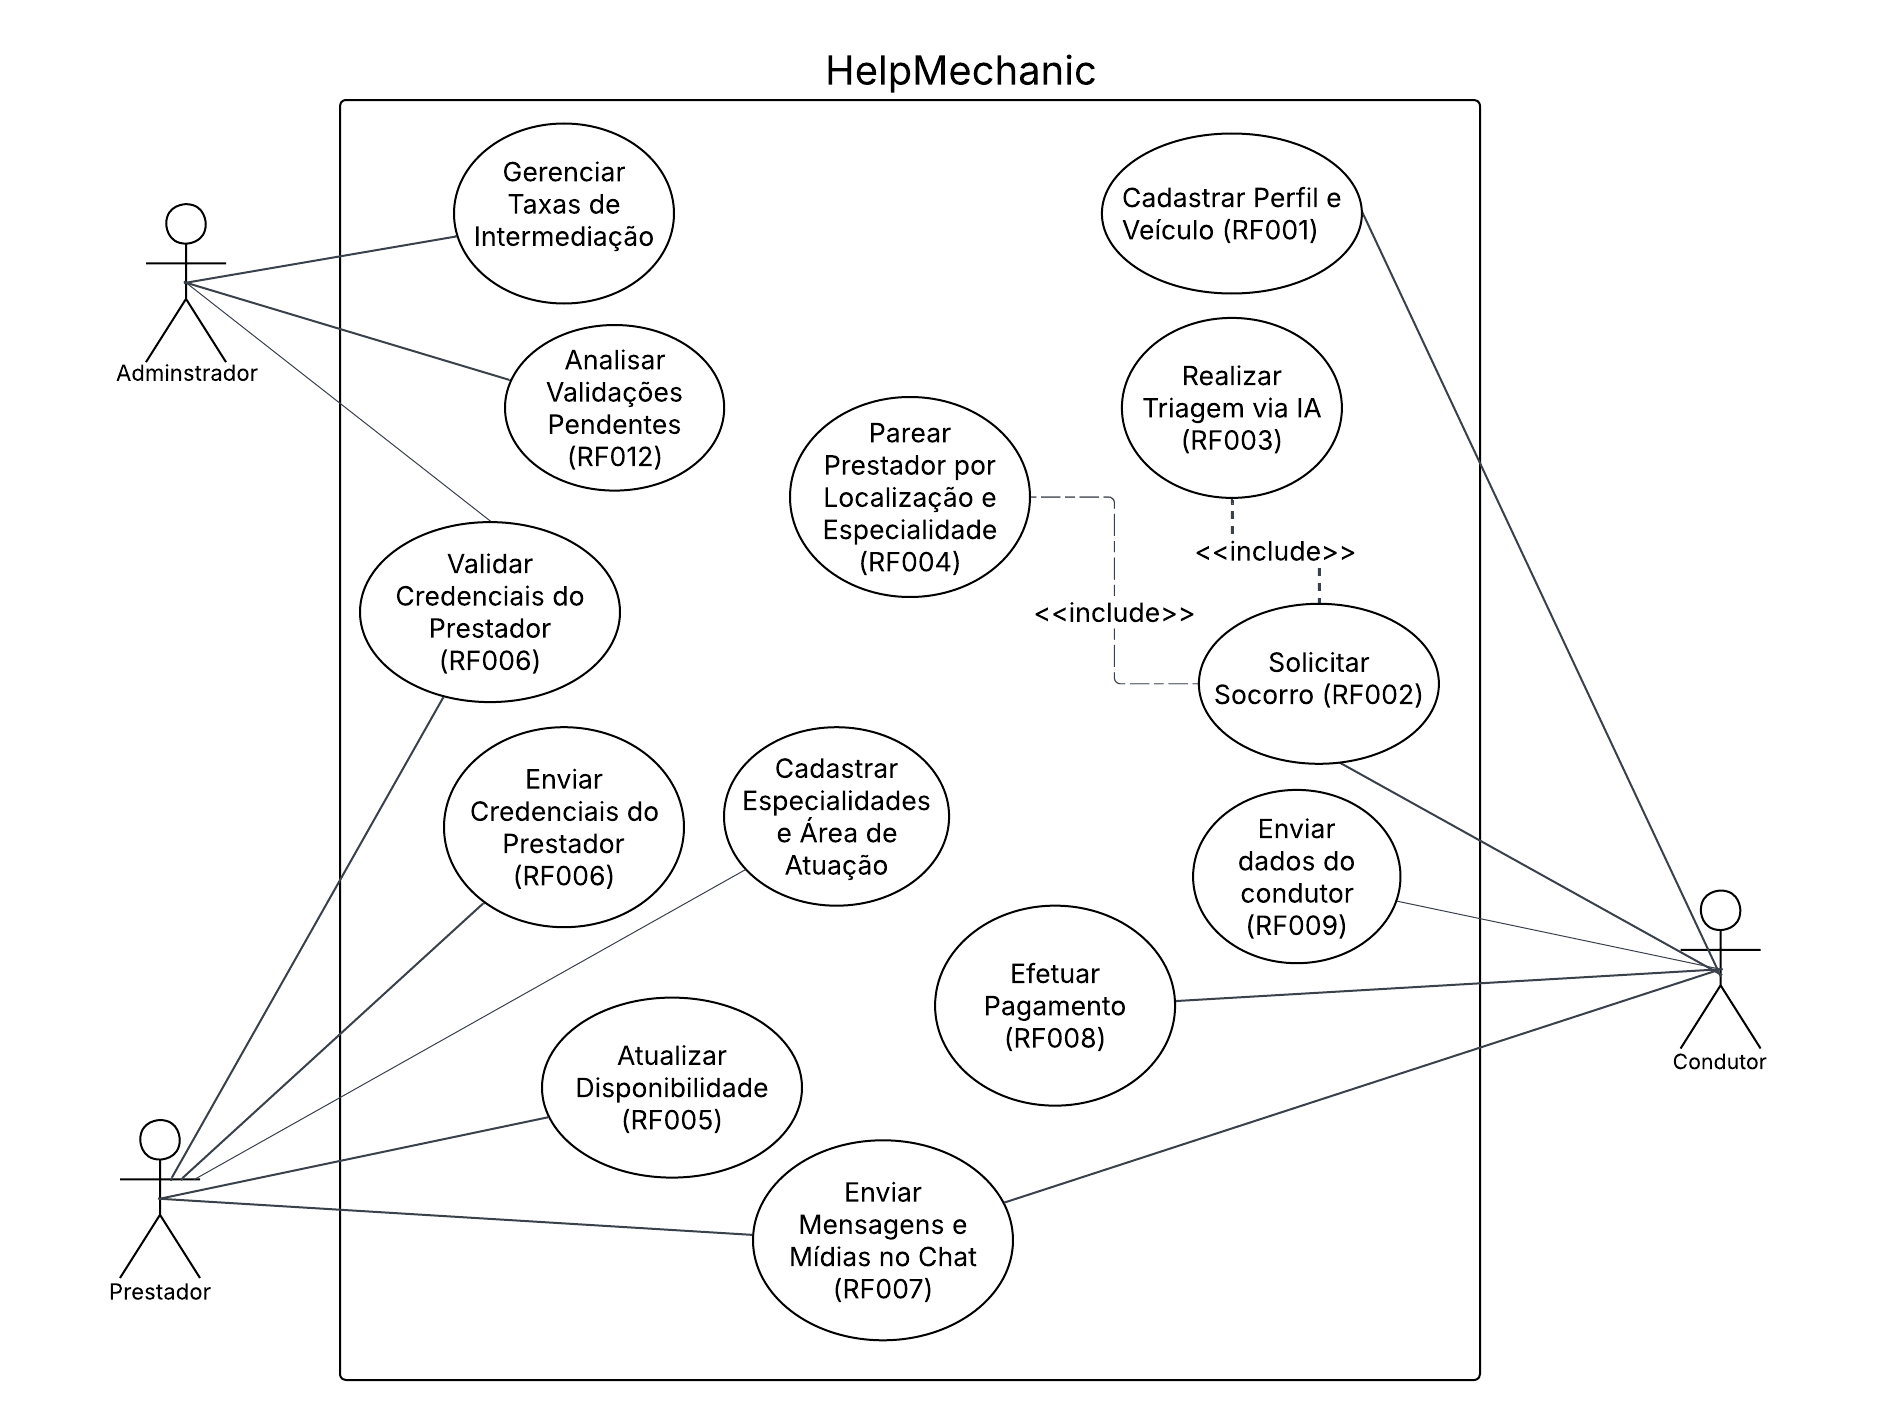
\includegraphics[width=0.98\linewidth]{diagrama_uml.png}
    \caption{Diagrama de caso de uso UML do sistema HelpMechanic.}
    \label{fig:caso_uso_helpmechanic}
\end{figure}

\subsection{Fluxograma}
em desenvolvimento

\subsection{Modelo Relacional}
em desenvolvimento

\subsection{Principais Telas do Sistema}
em desenvolvimento

\section{Conclusões}
Este trabalho apresentou a especificação inicial do HelpMechanic, uma plataforma móvel voltada à intermediação de serviços de socorro mecânico e borracharia em Paranaguá-PR. A proposta demonstrou-se relevante diante do contexto urbano e logístico local, marcado pela circulação intensa de veículos leves e pesados e pela necessidade de respostas rápidas em situações de falha veicular. Como contribuição, foram definidos requisitos funcionais, requisitos não funcionais, regras de negócio e elementos iniciais de arquitetura, contemplando geolocalização, triagem assistida por IA, validação de identidade e pareamento por proximidade e especialidade técnica.

Apesar disso, o trabalho ainda se encontra em estágio de especificação e prototipação, não permitindo afirmar de forma conclusiva a redução do tempo de imobilização veicular. Dessa forma, a validação do sistema em ambiente real, com usuários e prestadores, constitui etapa essencial para verificar sua efetividade, usabilidade e desempenho em cenários de baixa conectividade.

\subsection{Trabalhos Futuros}
Como trabalhos futuros, propõe-se a implementação completa do protótipo funcional, a validação do algoritmo de pareamento com dados reais, a realização de testes de usabilidade com condutores e prestadores, a integração com serviços externos de validação de identidade e a avaliação do desempenho da aplicação em cenários de baixa conectividade. Também se recomenda aprofundar os mecanismos de privacidade, auditoria e retenção de dados, considerando os requisitos da LGPD \cite{brasil_lgpd2018} e a segurança dos participantes da plataforma.

\bibliographystyle{sbc}
\bibliography{references}

\end{document}
